
\begin{frame}
  \frametitle{Benchmarking : Single Tunnel Case, Peak Heat}
For the single tunnel geometry benchmark, the 
analytic model gave peak temperatures for all cases run which agreed with the 
numeric model within $4^{\circ}C$ and, for calculation radii less than 5 meters.

\footnotesize{
\begin{table}
  \centering
  \begin{tabular}{|l|l|l|l|l|l|l|}
    \multicolumn{7}{c}{\textbf{Benchmarking Results for Single Tunnel 
    Scenario}}\\
    \hline
    & \multicolumn{6}{|c|}{Peak Temperature Discrepancy}\\ 
    & \multicolumn{6}{|c|}{$T_{peak,num}-T_{peak,an}$ $[^{\circ}C]$} \\
    \hline
    Material & \multicolumn{3}{|c|}{Clay} & \multicolumn{3}{|c|}{Salt}\\ & 
    \multicolumn{3}{|c|}{$K_{th}=2.5$} & \multicolumn{3}{|c|}{$K_{th}=4.2$}\\ & 
    \multicolumn{3}{|c|}{$\alpha=1.13\times10^{-6}$} & 
    \multicolumn{3}{|c|}{$\alpha=2.07\times10^{-6}$}\\ 
    \hline
    Years Cooling  & 10     & 25      & 50      & 10     & 25     & 50\\
    \hline
     R=0.35m  & 3.0   & 2.3     & 1.6    & 2.0   & 1.7   & 1.2\\
     R=0.69m  & 3.1   & 2.4    & 1.6    & 2.2    & 1.8   & 1.3\\
     R=3.46m  & 2.1   & 1.9    & 1.5    & 2.2   & 1.7    & 1.3\\
    \hline
  \end{tabular}
  \caption{Benchmarking in the single tunnel case showed that the peak heat was 
  calculated to be lower and arrived consistently sooner in the analytic (an) 
  model than in the numeric (num) model.  }
\end{table}
}
\end{frame}

\begin{frame}
  \frametitle{Benchmarking : Single Tunnel Case, Timing}
For the single tunnel geometry benchmark, the analytic model
consistently reported peak temperature timing within 11 years of the ANL 
numeric model. 
\footnotesize{
\begin{table}
  \begin{centering}
  \begin{tabular}{|l|l|l|l|l|l|l|}
    \multicolumn{7}{c}{\textbf{Benchmarking Results for Single Tunnel 
    Scenario}}\\
    \hline
    & \multicolumn{6}{|c|}{Peak Heat Timing Discrepancy}\\ 
    & \multicolumn{6}{|c|}{ $t_{peak,num}-t_{peak,an}$ [yr]} \\
    \hline
    Material & \multicolumn{3}{|c|}{Clay} & \multicolumn{3}{|c|}{Salt}\\ & 
    \multicolumn{3}{|c|}{$K_{th}=2.5$} & \multicolumn{3}{|c|}{$K_{th}=4.2$}\\ & 
    \multicolumn{3}{|c|}{$\alpha=1.13\times10^{-6}$} & 
    \multicolumn{3}{|c|}{$\alpha=2.07\times10^{-6}$}\\ \hline
    Years Cooling  & 10     & 25      & 50      & 10     & 25     & 50\\
    \hline
     R=0.35m  & 1    & 1       & 1   & 1      & 1      & 3\\
     R=0.69m  & 2    & 2       & 1    & 2      & 3      & 4\\
     R=3.46m  & 9    & 7       & 6    & 4      & 2      & 11\\
    \hline
  \end{tabular}
  \caption{Benchmarking in the single tunnel case showed that the peak heat was 
  calculated to be lower and arrived consistently sooner in the analytic (an) 
  model than in the numeric (num) model.  }
  \label{tab:benchSingle}
\end{centering}
\end{table}
}
\end{frame}

\begin{frame}
  \frametitle{Benchmarking : Single Tunnel Case, Clay}
    \begin{figure}[h]
      \begin{center}
        \includegraphics[width=\textwidth]{1Drift1UOXWFLLNL_Clay10yr.eps}
      \end{center}
      \caption{UOX waste form, 10 years cooling, clay scenario.}
      \label{fig:10clay}
    \end{figure}
\end{frame}

\begin{frame}
  \frametitle{Benchmarking : Single Tunnel Case, Salt}
    \begin{figure}[h]
      \begin{center}
        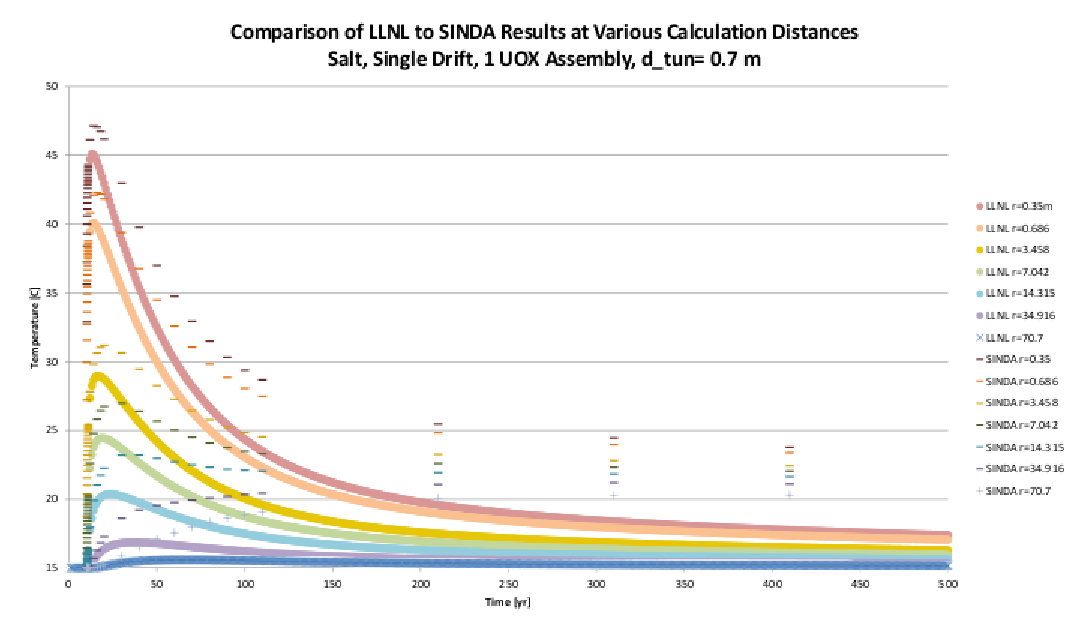
\includegraphics[width=\textwidth]{1Drift1UOXWFLLNL_Salt10yr.eps}
      \end{center}
      \caption{UOX waste form, 10 years cooling, salt scenario.}
      \label{fig:10salt}
    \end{figure}
\end{frame}

\begin{frame}
  \frametitle{Benchmarking : Multiple Tunnel Case }
For the multiple tunnel case, in which the numeric model 
approximated an infinite array of tunnels and the analytic approach modeled 101, 
the differences between models were slightly greater. 
\begin{table}
  \centering
  \footnotesize{
  \begin{tabular}{|l|l|l|l|}
    \multicolumn{4}{c}{\textbf{Benchmarking Results for 101 Tunnel Scenario}}\\
    \hline
    Material & \multicolumn{3}{|c|}{Clay} \\
    & \multicolumn{3}{|c|}{$K_{th}=2.5$}\\ 
    & \multicolumn{3}{|c|}{$\alpha=1.13\times10^{-6}$}  \\
    \hline
    & \multicolumn{3}{|c|}{Peak Temperature Discrepancy} \\
    & \multicolumn{3}{|c|}{$T_{peak,num}-T_{peak,an}$ $[^{\circ}C]$} \\
    \hline
    Years Cooling  & 10  & 25 & 50 \\
    \hline
    R=0.35m   & 7 & 4.6 & 2.1 \\
    \hline
    &\multicolumn{3}{|c|}{Peak Heat Timing Discrepancy}\\
    &\multicolumn{3}{|c|}{ $t_{peak,num}-t_{peak,an}$ [yr]} \\
    \hline
    R=0.35m       & -13.5   & 2   & -6  \\
    \hline
  \end{tabular}
  \caption{Benchmarking in the multiple tunnel case showed that the peak heat was 
  calculated to be consistently lower in the analytic (an) model and deviated further
  from the numeric (num)  model than did the single tunnel case.
  }
  \label{tab:benchMulti}
  }
\end{table}

\end{frame}


\begin{frame}
  \frametitle{Benchmarking : Summary}

In light of the magnitude of uncertainties involved in generically modeling a 
non-site-specific geologic repository, this sufficiently validated the analytic 
LLNL model with respect to its goals.  The analytic model would seem 
well-suited for purposes of rapid evaluation of generic geologic repository 
configurations. 

The benchmark revealed a notable discrepancy between the two models, 
however. The time of peak heat arrived consistently sooner and the value of the 
peak temperature was consistently lower in the homogeneous medium analytic
model than in the numeric model. 
\end{frame}

